\documentclass[twoside]{book}

% Packages required by doxygen
\usepackage{fixltx2e}
\usepackage{calc}
\usepackage{doxygen}
\usepackage[export]{adjustbox} % also loads graphicx
\usepackage{graphicx}
\usepackage[utf8]{inputenc}
\usepackage{makeidx}
\usepackage{multicol}
\usepackage{multirow}
\PassOptionsToPackage{warn}{textcomp}
\usepackage{textcomp}
\usepackage[nointegrals]{wasysym}
\usepackage[table]{xcolor}

% Font selection
\usepackage[T1]{fontenc}
\usepackage[scaled=.90]{helvet}
\usepackage{courier}
\usepackage{amssymb}
\usepackage{sectsty}
\renewcommand{\familydefault}{\sfdefault}
\allsectionsfont{%
  \fontseries{bc}\selectfont%
  \color{darkgray}%
}
\renewcommand{\DoxyLabelFont}{%
  \fontseries{bc}\selectfont%
  \color{darkgray}%
}
\newcommand{\+}{\discretionary{\mbox{\scriptsize$\hookleftarrow$}}{}{}}

% Page & text layout
\usepackage{geometry}
\geometry{%
  a4paper,%
  top=2.5cm,%
  bottom=2.5cm,%
  left=2.5cm,%
  right=2.5cm%
}
\tolerance=750
\hfuzz=15pt
\hbadness=750
\setlength{\emergencystretch}{15pt}
\setlength{\parindent}{0cm}
\setlength{\parskip}{3ex plus 2ex minus 2ex}
\makeatletter
\renewcommand{\paragraph}{%
  \@startsection{paragraph}{4}{0ex}{-1.0ex}{1.0ex}{%
    \normalfont\normalsize\bfseries\SS@parafont%
  }%
}
\renewcommand{\subparagraph}{%
  \@startsection{subparagraph}{5}{0ex}{-1.0ex}{1.0ex}{%
    \normalfont\normalsize\bfseries\SS@subparafont%
  }%
}
\makeatother

% Headers & footers
\usepackage{fancyhdr}
\pagestyle{fancyplain}
\fancyhead[LE]{\fancyplain{}{\bfseries\thepage}}
\fancyhead[CE]{\fancyplain{}{}}
\fancyhead[RE]{\fancyplain{}{\bfseries\leftmark}}
\fancyhead[LO]{\fancyplain{}{\bfseries\rightmark}}
\fancyhead[CO]{\fancyplain{}{}}
\fancyhead[RO]{\fancyplain{}{\bfseries\thepage}}
\fancyfoot[LE]{\fancyplain{}{}}
\fancyfoot[CE]{\fancyplain{}{}}
\fancyfoot[RE]{\fancyplain{}{\bfseries\scriptsize Generated by Doxygen }}
\fancyfoot[LO]{\fancyplain{}{\bfseries\scriptsize Generated by Doxygen }}
\fancyfoot[CO]{\fancyplain{}{}}
\fancyfoot[RO]{\fancyplain{}{}}
\renewcommand{\footrulewidth}{0.4pt}
\renewcommand{\chaptermark}[1]{%
  \markboth{#1}{}%
}
\renewcommand{\sectionmark}[1]{%
  \markright{\thesection\ #1}%
}

% Indices & bibliography
\usepackage{natbib}
\usepackage[titles]{tocloft}
\setcounter{tocdepth}{3}
\setcounter{secnumdepth}{5}
\makeindex

% Hyperlinks (required, but should be loaded last)
\usepackage{ifpdf}
\ifpdf
  \usepackage[pdftex,pagebackref=true]{hyperref}
\else
  \usepackage[ps2pdf,pagebackref=true]{hyperref}
\fi
\hypersetup{%
  colorlinks=true,%
  linkcolor=blue,%
  citecolor=blue,%
  unicode%
}

% Custom commands
\newcommand{\clearemptydoublepage}{%
  \newpage{\pagestyle{empty}\cleardoublepage}%
}

\usepackage{caption}
\captionsetup{labelsep=space,justification=centering,font={bf},singlelinecheck=off,skip=4pt,position=top}

%===== C O N T E N T S =====

\begin{document}

% Titlepage & ToC
\hypersetup{pageanchor=false,
             bookmarksnumbered=true,
             pdfencoding=unicode
            }
\pagenumbering{alph}
\begin{titlepage}
\vspace*{7cm}
\begin{center}%
{\Large Exploration }\\
\vspace*{1cm}
{\large Generated by Doxygen 1.8.12}\\
\end{center}
\end{titlepage}
\clearemptydoublepage
\pagenumbering{roman}
\tableofcontents
\clearemptydoublepage
\pagenumbering{arabic}
\hypersetup{pageanchor=true}

%--- Begin generated contents ---
\chapter{Hierarchical Index}
\section{Class Hierarchy}
This inheritance list is sorted roughly, but not completely, alphabetically\+:\begin{DoxyCompactList}
\item \contentsline{section}{radiation\+:\+:Belief\+Error}{\pageref{structradiation_1_1_belief_error}}{}
\item \contentsline{section}{radiation\+:\+:Belief\+Regularization}{\pageref{structradiation_1_1_belief_regularization}}{}
\item \contentsline{section}{radiation\+:\+:Explorer2D}{\pageref{classradiation_1_1_explorer2_d}}{}
\begin{DoxyCompactList}
\item \contentsline{section}{radiation\+:\+:Explorer\+LP}{\pageref{classradiation_1_1_explorer_l_p}}{}
\item \contentsline{section}{radiation\+:\+:Explorer\+RW}{\pageref{classradiation_1_1_explorer_r_w}}{}
\item \contentsline{section}{radiation\+:\+:Explorer\+S\+O\+CP}{\pageref{classradiation_1_1_explorer_s_o_c_p}}{}
\end{DoxyCompactList}
\item \contentsline{section}{radiation\+:\+:Grid\+Map2D}{\pageref{classradiation_1_1_grid_map2_d}}{}
\item \contentsline{section}{radiation\+:\+:Grid\+Pose2D}{\pageref{classradiation_1_1_grid_pose2_d}}{}
\item \contentsline{section}{radiation\+:\+:Movement2D}{\pageref{classradiation_1_1_movement2_d}}{}
\item \contentsline{section}{radiation\+:\+:Problem2D}{\pageref{classradiation_1_1_problem2_d}}{}
\item \contentsline{section}{radiation\+:\+:Sensor2D}{\pageref{classradiation_1_1_sensor2_d}}{}
\item \contentsline{section}{radiation\+:\+:Source2D}{\pageref{classradiation_1_1_source2_d}}{}
\end{DoxyCompactList}

\chapter{Class Index}
\section{Class List}
Here are the classes, structs, unions and interfaces with brief descriptions\+:\begin{DoxyCompactList}
\item\contentsline{section}{\hyperlink{structradiation_1_1_belief_error}{radiation\+::\+Belief\+Error} }{\pageref{structradiation_1_1_belief_error}}{}
\item\contentsline{section}{\hyperlink{structradiation_1_1_belief_regularization}{radiation\+::\+Belief\+Regularization} }{\pageref{structradiation_1_1_belief_regularization}}{}
\item\contentsline{section}{\hyperlink{classradiation_1_1_explorer2_d}{radiation\+::\+Explorer2D} }{\pageref{classradiation_1_1_explorer2_d}}{}
\item\contentsline{section}{\hyperlink{classradiation_1_1_explorer_l_p}{radiation\+::\+Explorer\+LP} }{\pageref{classradiation_1_1_explorer_l_p}}{}
\item\contentsline{section}{\hyperlink{classradiation_1_1_explorer_r_w}{radiation\+::\+Explorer\+RW} }{\pageref{classradiation_1_1_explorer_r_w}}{}
\item\contentsline{section}{\hyperlink{classradiation_1_1_explorer_s_o_c_p}{radiation\+::\+Explorer\+S\+O\+CP} }{\pageref{classradiation_1_1_explorer_s_o_c_p}}{}
\item\contentsline{section}{\hyperlink{classradiation_1_1_grid_map2_d}{radiation\+::\+Grid\+Map2D} }{\pageref{classradiation_1_1_grid_map2_d}}{}
\item\contentsline{section}{\hyperlink{classradiation_1_1_grid_pose2_d}{radiation\+::\+Grid\+Pose2D} }{\pageref{classradiation_1_1_grid_pose2_d}}{}
\item\contentsline{section}{\hyperlink{classradiation_1_1_movement2_d}{radiation\+::\+Movement2D} }{\pageref{classradiation_1_1_movement2_d}}{}
\item\contentsline{section}{\hyperlink{classradiation_1_1_problem2_d}{radiation\+::\+Problem2D} }{\pageref{classradiation_1_1_problem2_d}}{}
\item\contentsline{section}{\hyperlink{classradiation_1_1_sensor2_d}{radiation\+::\+Sensor2D} }{\pageref{classradiation_1_1_sensor2_d}}{}
\item\contentsline{section}{\hyperlink{classradiation_1_1_source2_d}{radiation\+::\+Source2D} }{\pageref{classradiation_1_1_source2_d}}{}
\end{DoxyCompactList}

\chapter{Class Documentation}
\hypertarget{structradiation_1_1_belief_error}{}\section{radiation\+:\+:Belief\+Error Struct Reference}
\label{structradiation_1_1_belief_error}\index{radiation\+::\+Belief\+Error@{radiation\+::\+Belief\+Error}}
\subsection*{Public Member Functions}
\begin{DoxyCompactItemize}
\item 
\hypertarget{structradiation_1_1_belief_error_afe05bfba363694b7875347da9527ba60}{}\label{structradiation_1_1_belief_error_afe05bfba363694b7875347da9527ba60} 
{\bfseries Belief\+Error} (const std\+::vector$<$ unsigned int $>$ $\ast$voxels, unsigned int measurement)
\item 
\hypertarget{structradiation_1_1_belief_error_ae6f3fb3e795a255e840ce37f7765a43d}{}\label{structradiation_1_1_belief_error_ae6f3fb3e795a255e840ce37f7765a43d} 
{\footnotesize template$<$typename T $>$ }\\bool {\bfseries operator()} (T const $\ast$const $\ast$belief, T $\ast$expected\+\_\+error) const
\end{DoxyCompactItemize}
\subsection*{Static Public Member Functions}
\begin{DoxyCompactItemize}
\item 
\hypertarget{structradiation_1_1_belief_error_ab6efeeae21abcfeb7897dc5310193577}{}\label{structradiation_1_1_belief_error_ab6efeeae21abcfeb7897dc5310193577} 
static ceres\+::\+Cost\+Function $\ast$ {\bfseries Create} (unsigned int num\+\_\+rows, unsigned int num\+\_\+cols, const std\+::vector$<$ unsigned int $>$ $\ast$voxels, const unsigned int measurement)
\end{DoxyCompactItemize}
\subsection*{Public Attributes}
\begin{DoxyCompactItemize}
\item 
\hypertarget{structradiation_1_1_belief_error_ae74f7c931d6e53006d17ad6768f1a289}{}\label{structradiation_1_1_belief_error_ae74f7c931d6e53006d17ad6768f1a289} 
const std\+::vector$<$ unsigned int $>$ $\ast$ {\bfseries voxels\+\_\+}
\item 
\hypertarget{structradiation_1_1_belief_error_a8bd1d2963e7729c0abafa3592a1571b7}{}\label{structradiation_1_1_belief_error_a8bd1d2963e7729c0abafa3592a1571b7} 
const unsigned int {\bfseries measurement\+\_\+}
\end{DoxyCompactItemize}


\subsection{Detailed Description}


Definition at line 66 of file cost\+\_\+functors.\+h.



The documentation for this struct was generated from the following file\+:\begin{DoxyCompactItemize}
\item 
/\+Users/davidfridovichkeil/\+Documents/\+Developer/exploration/radiation/cpp/include/cost\+\_\+functors.\+h\end{DoxyCompactItemize}

\hypertarget{structradiation_1_1_belief_regularization}{}\section{radiation\+:\+:Belief\+Regularization Struct Reference}
\label{structradiation_1_1_belief_regularization}\index{radiation\+::\+Belief\+Regularization@{radiation\+::\+Belief\+Regularization}}
\subsection*{Public Member Functions}
\begin{DoxyCompactItemize}
\item 
\hypertarget{structradiation_1_1_belief_regularization_a299b47bdef4ef20a980376ffc6dad3f7}{}\label{structradiation_1_1_belief_regularization_a299b47bdef4ef20a980376ffc6dad3f7} 
{\bfseries Belief\+Regularization} (unsigned int num\+\_\+parameters, int num\+\_\+sources, double regularizer)
\item 
\hypertarget{structradiation_1_1_belief_regularization_a037b7fcffbf148759e087a1c645ba6be}{}\label{structradiation_1_1_belief_regularization_a037b7fcffbf148759e087a1c645ba6be} 
{\footnotesize template$<$typename T $>$ }\\bool {\bfseries operator()} (T const $\ast$const $\ast$belief, T $\ast$expected\+\_\+error) const
\end{DoxyCompactItemize}
\subsection*{Static Public Member Functions}
\begin{DoxyCompactItemize}
\item 
\hypertarget{structradiation_1_1_belief_regularization_af0b266b48c16d621b921b86ecdb4a406}{}\label{structradiation_1_1_belief_regularization_af0b266b48c16d621b921b86ecdb4a406} 
static ceres\+::\+Cost\+Function $\ast$ {\bfseries Create} (unsigned int num\+\_\+rows, unsigned int num\+\_\+cols, unsigned int num\+\_\+sources, double regularizer)
\end{DoxyCompactItemize}
\subsection*{Public Attributes}
\begin{DoxyCompactItemize}
\item 
\hypertarget{structradiation_1_1_belief_regularization_aca8f44de0a47d50a25a79084bb871d82}{}\label{structradiation_1_1_belief_regularization_aca8f44de0a47d50a25a79084bb871d82} 
const unsigned int {\bfseries num\+\_\+parameters\+\_\+}
\item 
\hypertarget{structradiation_1_1_belief_regularization_ae3ae44194d0a343720ae0a2469949dca}{}\label{structradiation_1_1_belief_regularization_ae3ae44194d0a343720ae0a2469949dca} 
const unsigned int {\bfseries num\+\_\+sources\+\_\+}
\item 
\hypertarget{structradiation_1_1_belief_regularization_a791c0ddeda2af95d559ed3c4b11b6abb}{}\label{structradiation_1_1_belief_regularization_a791c0ddeda2af95d559ed3c4b11b6abb} 
const double {\bfseries regularizer\+\_\+}
\end{DoxyCompactItemize}


\subsection{Detailed Description}


Definition at line 119 of file cost\+\_\+functors.\+h.



The documentation for this struct was generated from the following file\+:\begin{DoxyCompactItemize}
\item 
/\+Users/davidfridovichkeil/\+Documents/\+Developer/exploration/radiation/cpp/include/cost\+\_\+functors.\+h\end{DoxyCompactItemize}

\hypertarget{classradiation_1_1_explorer2_d}{}\section{radiation\+:\+:Explorer2D Class Reference}
\label{classradiation_1_1_explorer2_d}\index{radiation\+::\+Explorer2D@{radiation\+::\+Explorer2D}}
Inheritance diagram for radiation\+:\+:Explorer2D\+:\begin{figure}[H]
\begin{center}
\leavevmode
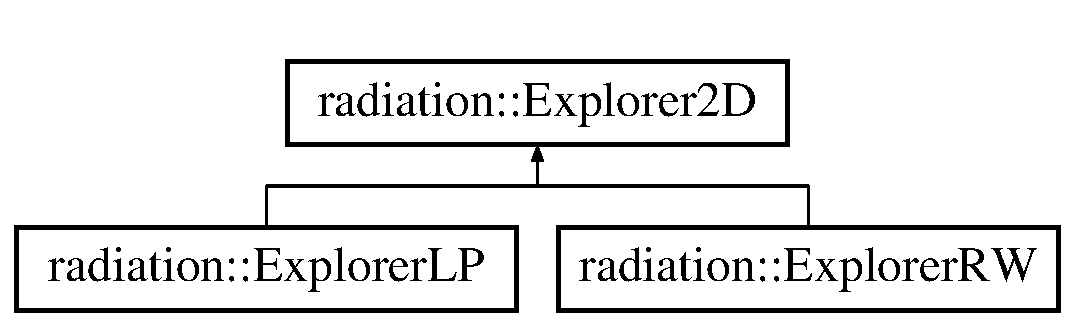
\includegraphics[height=2.000000cm]{classradiation_1_1_explorer2_d}
\end{center}
\end{figure}
\subsection*{Public Member Functions}
\begin{DoxyCompactItemize}
\item 
\hypertarget{classradiation_1_1_explorer2_d_a7caa50fec51ce47cf9ee96400496b334}{}\label{classradiation_1_1_explorer2_d_a7caa50fec51ce47cf9ee96400496b334} 
{\bfseries Explorer2D} (unsigned int num\+\_\+rows, unsigned int num\+\_\+cols, unsigned int num\+\_\+sources, double regularizer, double fov, const std\+::vector$<$ \hyperlink{classradiation_1_1_source2_d}{Source2D} $>$ \&sources, const \hyperlink{classradiation_1_1_grid_pose2_d}{Grid\+Pose2D} \&initial\+\_\+pose)
\item 
\hypertarget{classradiation_1_1_explorer2_d_ad16e982f1455a8813c02e4efbbfbdc29}{}\label{classradiation_1_1_explorer2_d_ad16e982f1455a8813c02e4efbbfbdc29} 
{\bfseries Explorer2D} (unsigned int num\+\_\+rows, unsigned int num\+\_\+cols, unsigned int num\+\_\+sources, double regularizer, double fov)
\item 
\hypertarget{classradiation_1_1_explorer2_d_a383dd22050fca3ee0bd47f746f571189}{}\label{classradiation_1_1_explorer2_d_a383dd22050fca3ee0bd47f746f571189} 
virtual bool {\bfseries Plan\+Ahead} (std\+::vector$<$ \hyperlink{classradiation_1_1_grid_pose2_d}{Grid\+Pose2D} $>$ \&trajectory)=0
\item 
\hypertarget{classradiation_1_1_explorer2_d_a406e0a334d57aa05cf1a37bcd4b1fcec}{}\label{classradiation_1_1_explorer2_d_a406e0a334d57aa05cf1a37bcd4b1fcec} 
double {\bfseries Take\+Step} (const std\+::vector$<$ \hyperlink{classradiation_1_1_grid_pose2_d}{Grid\+Pose2D} $>$ \&trajectory)
\item 
\hypertarget{classradiation_1_1_explorer2_d_ac78860771fe00720a8024ef06a1b13b3}{}\label{classradiation_1_1_explorer2_d_ac78860771fe00720a8024ef06a1b13b3} 
double {\bfseries Entropy} () const
\item 
\hypertarget{classradiation_1_1_explorer2_d_a8eaf1135c2d720ac185b4afbb852feee}{}\label{classradiation_1_1_explorer2_d_a8eaf1135c2d720ac185b4afbb852feee} 
void {\bfseries Visualize} () const
\end{DoxyCompactItemize}
\subsection*{Protected Attributes}
\begin{DoxyCompactItemize}
\item 
\hypertarget{classradiation_1_1_explorer2_d_a67746d1bf33ea4a0f9d5794e490a9d40}{}\label{classradiation_1_1_explorer2_d_a67746d1bf33ea4a0f9d5794e490a9d40} 
double {\bfseries fov\+\_\+}
\item 
\hypertarget{classradiation_1_1_explorer2_d_ad9d295085a98c134f54fc2acf9f6c3b9}{}\label{classradiation_1_1_explorer2_d_ad9d295085a98c134f54fc2acf9f6c3b9} 
\hyperlink{classradiation_1_1_grid_map2_d}{Grid\+Map2D} {\bfseries map\+\_\+}
\item 
\hypertarget{classradiation_1_1_explorer2_d_ad178dd47cb8778f1c99a7a600d5ca625}{}\label{classradiation_1_1_explorer2_d_ad178dd47cb8778f1c99a7a600d5ca625} 
\hyperlink{classradiation_1_1_grid_pose2_d}{Grid\+Pose2D} {\bfseries pose\+\_\+}
\item 
\hypertarget{classradiation_1_1_explorer2_d_a89003d6709bf9d0f5b09bc561e1d50ce}{}\label{classradiation_1_1_explorer2_d_a89003d6709bf9d0f5b09bc561e1d50ce} 
std\+::vector$<$ \hyperlink{classradiation_1_1_source2_d}{Source2D} $>$ {\bfseries sources\+\_\+}
\item 
\hypertarget{classradiation_1_1_explorer2_d_ae221c334df98e0676a49ab678124749e}{}\label{classradiation_1_1_explorer2_d_ae221c334df98e0676a49ab678124749e} 
std\+::vector$<$ \hyperlink{classradiation_1_1_grid_pose2_d}{Grid\+Pose2D} $>$ {\bfseries past\+\_\+poses\+\_\+}
\end{DoxyCompactItemize}


\subsection{Detailed Description}


Definition at line 60 of file explorer\+\_\+2d.\+h.



The documentation for this class was generated from the following files\+:\begin{DoxyCompactItemize}
\item 
/\+Users/davidfridovichkeil/\+Documents/\+Developer/exploration/radiation/cpp/include/explorer\+\_\+2d.\+h\item 
/\+Users/davidfridovichkeil/\+Documents/\+Developer/exploration/radiation/cpp/src/explorer\+\_\+2d.\+cpp\end{DoxyCompactItemize}

\hypertarget{classradiation_1_1_explorer_l_p}{}\section{radiation\+:\+:Explorer\+LP Class Reference}
\label{classradiation_1_1_explorer_l_p}\index{radiation\+::\+Explorer\+LP@{radiation\+::\+Explorer\+LP}}
Inheritance diagram for radiation\+:\+:Explorer\+LP\+:\begin{figure}[H]
\begin{center}
\leavevmode
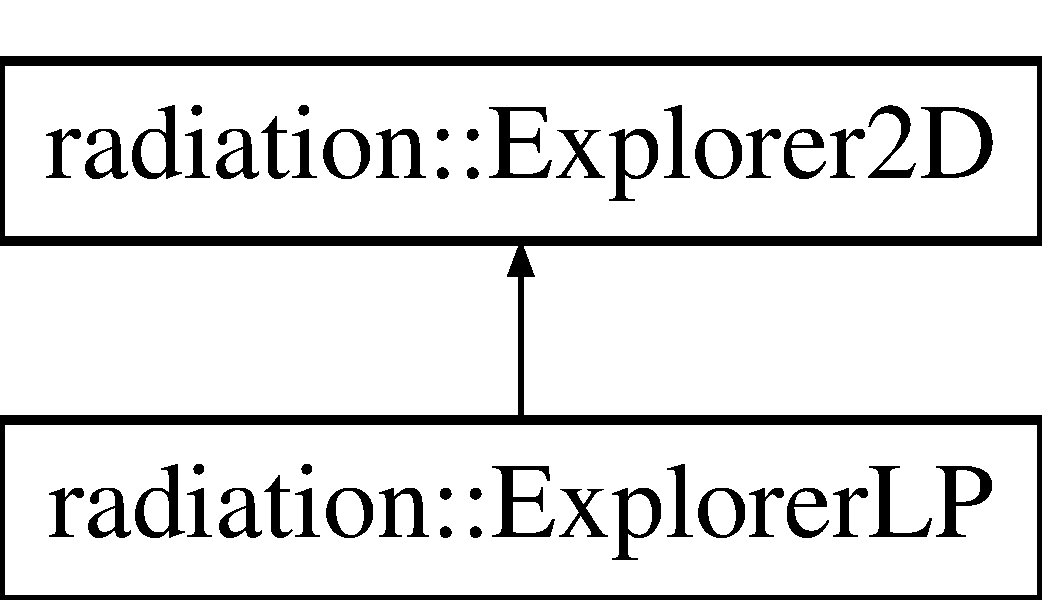
\includegraphics[height=2.000000cm]{classradiation_1_1_explorer_l_p}
\end{center}
\end{figure}
\subsection*{Public Member Functions}
\begin{DoxyCompactItemize}
\item 
\hypertarget{classradiation_1_1_explorer_l_p_ac650cf72509513325bb4672fa97dd6ae}{}\label{classradiation_1_1_explorer_l_p_ac650cf72509513325bb4672fa97dd6ae} 
{\bfseries Explorer\+LP} (unsigned int num\+\_\+rows, unsigned int num\+\_\+cols, unsigned int num\+\_\+sources, double regularizer, unsigned int num\+\_\+steps, double fov, unsigned int num\+\_\+samples, const std\+::vector$<$ \hyperlink{classradiation_1_1_source2_d}{Source2D} $>$ \&sources, const \hyperlink{classradiation_1_1_grid_pose2_d}{Grid\+Pose2D} \&initial\+\_\+pose)
\item 
\hypertarget{classradiation_1_1_explorer_l_p_a3d37154001011ae4a81c5ee7d26b8f62}{}\label{classradiation_1_1_explorer_l_p_a3d37154001011ae4a81c5ee7d26b8f62} 
{\bfseries Explorer\+LP} (unsigned int num\+\_\+rows, unsigned int num\+\_\+cols, unsigned int num\+\_\+sources, double regularizer, unsigned int num\+\_\+steps, double fov, unsigned int num\+\_\+samples)
\item 
\hypertarget{classradiation_1_1_explorer_l_p_accde83eac496f12dede4737b8a57ce51}{}\label{classradiation_1_1_explorer_l_p_accde83eac496f12dede4737b8a57ce51} 
bool {\bfseries Plan\+Ahead} (std\+::vector$<$ \hyperlink{classradiation_1_1_grid_pose2_d}{Grid\+Pose2D} $>$ \&trajectory)
\end{DoxyCompactItemize}
\subsection*{Additional Inherited Members}


\subsection{Detailed Description}


Definition at line 53 of file explorer\+\_\+lp.\+h.



The documentation for this class was generated from the following files\+:\begin{DoxyCompactItemize}
\item 
/\+Users/davidfridovichkeil/\+Documents/\+Developer/exploration/radiation/cpp/include/explorer\+\_\+lp.\+h\item 
/\+Users/davidfridovichkeil/\+Documents/\+Developer/exploration/radiation/cpp/src/explorer\+\_\+lp.\+cpp\end{DoxyCompactItemize}

\hypertarget{classradiation_1_1_explorer_r_w}{}\section{radiation\+:\+:Explorer\+RW Class Reference}
\label{classradiation_1_1_explorer_r_w}\index{radiation\+::\+Explorer\+RW@{radiation\+::\+Explorer\+RW}}
Inheritance diagram for radiation\+:\+:Explorer\+RW\+:\begin{figure}[H]
\begin{center}
\leavevmode
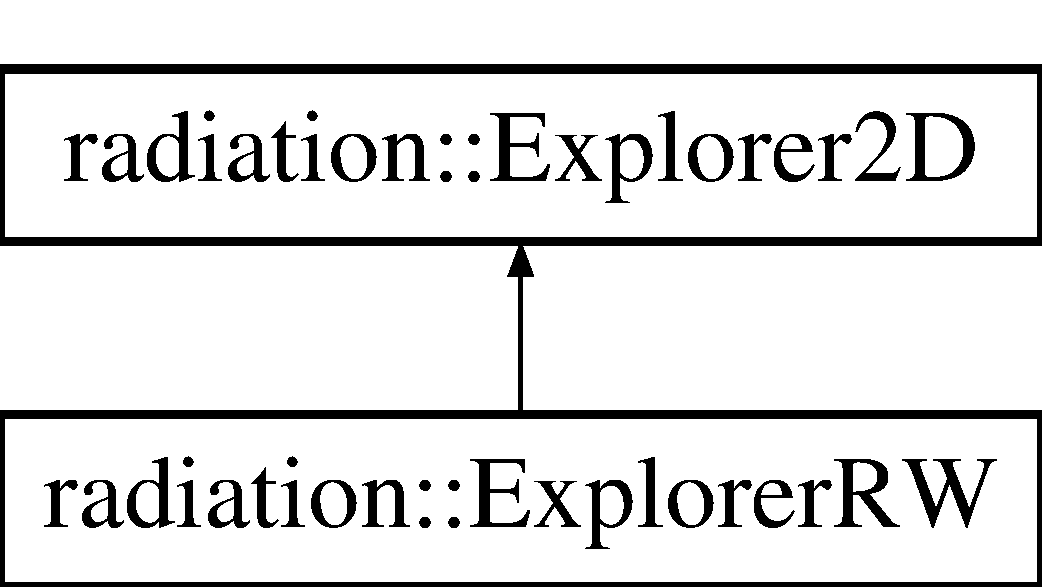
\includegraphics[height=2.000000cm]{classradiation_1_1_explorer_r_w}
\end{center}
\end{figure}
\subsection*{Public Member Functions}
\begin{DoxyCompactItemize}
\item 
\hypertarget{classradiation_1_1_explorer_r_w_aa1ea648af72ebcf4f4b82447545a1756}{}\label{classradiation_1_1_explorer_r_w_aa1ea648af72ebcf4f4b82447545a1756} 
{\bfseries Explorer\+RW} (unsigned int num\+\_\+rows, unsigned int num\+\_\+cols, unsigned int num\+\_\+sources, double regularizer, double fov, const std\+::vector$<$ \hyperlink{classradiation_1_1_source2_d}{Source2D} $>$ \&sources, const \hyperlink{classradiation_1_1_grid_pose2_d}{Grid\+Pose2D} \&initial\+\_\+pose)
\item 
\hypertarget{classradiation_1_1_explorer_r_w_a89a7d007495d2ac43f5863c59b25a97f}{}\label{classradiation_1_1_explorer_r_w_a89a7d007495d2ac43f5863c59b25a97f} 
{\bfseries Explorer\+RW} (unsigned int num\+\_\+rows, unsigned int num\+\_\+cols, unsigned int num\+\_\+sources, double regularizer, double fov)
\item 
\hypertarget{classradiation_1_1_explorer_r_w_a30e8acd62a435a5d424553412f219379}{}\label{classradiation_1_1_explorer_r_w_a30e8acd62a435a5d424553412f219379} 
bool {\bfseries Plan\+Ahead} (std\+::vector$<$ \hyperlink{classradiation_1_1_grid_pose2_d}{Grid\+Pose2D} $>$ \&trajectory)
\end{DoxyCompactItemize}
\subsection*{Additional Inherited Members}


\subsection{Detailed Description}


Definition at line 51 of file explorer\+\_\+rw.\+h.



The documentation for this class was generated from the following files\+:\begin{DoxyCompactItemize}
\item 
/\+Users/davidfridovichkeil/\+Documents/\+Developer/exploration/radiation/cpp/include/explorer\+\_\+rw.\+h\item 
/\+Users/davidfridovichkeil/\+Documents/\+Developer/exploration/radiation/cpp/src/explorer\+\_\+rw.\+cpp\end{DoxyCompactItemize}

\hypertarget{classradiation_1_1_grid_map2_d}{}\section{radiation\+:\+:Grid\+Map2D Class Reference}
\label{classradiation_1_1_grid_map2_d}\index{radiation\+::\+Grid\+Map2D@{radiation\+::\+Grid\+Map2D}}
\subsection*{Public Member Functions}
\begin{DoxyCompactItemize}
\item 
\hypertarget{classradiation_1_1_grid_map2_d_a7ffd2c7bd0b21ce282a8fa632c216129}{}\label{classradiation_1_1_grid_map2_d_a7ffd2c7bd0b21ce282a8fa632c216129} 
{\bfseries Grid\+Map2D} (unsigned int num\+\_\+rows, unsigned int num\+\_\+cols, unsigned int num\+\_\+sources, double regularizer)
\item 
\hypertarget{classradiation_1_1_grid_map2_d_a318bfa44824d9516c25281a3be8875eb}{}\label{classradiation_1_1_grid_map2_d_a318bfa44824d9516c25281a3be8875eb} 
unsigned int {\bfseries Get\+Num\+Rows} () const
\item 
\hypertarget{classradiation_1_1_grid_map2_d_abd22169061eabdfadc130e21dae4cbef}{}\label{classradiation_1_1_grid_map2_d_abd22169061eabdfadc130e21dae4cbef} 
unsigned int {\bfseries Get\+Num\+Cols} () const
\item 
\hypertarget{classradiation_1_1_grid_map2_d_a798ba7c6d39277a4b13002106b868817}{}\label{classradiation_1_1_grid_map2_d_a798ba7c6d39277a4b13002106b868817} 
bool {\bfseries Generate\+Sources} (std\+::vector$<$ \hyperlink{classradiation_1_1_source2_d}{Source2D} $>$ \&sources)
\item 
\hypertarget{classradiation_1_1_grid_map2_d_a3259e3877b8fecdb511e09762f1acdce}{}\label{classradiation_1_1_grid_map2_d_a3259e3877b8fecdb511e09762f1acdce} 
void {\bfseries Generate\+Entropy\+Vector} (unsigned int num\+\_\+samples, unsigned int num\+\_\+steps, const \hyperlink{classradiation_1_1_grid_pose2_d}{Grid\+Pose2D} \&pose, double sensor\+\_\+fov, Eigen\+::\+Vector\+Xd \&hzx, std\+::vector$<$ unsigned int $>$ \&trajectory\+\_\+ids)
\item 
\hypertarget{classradiation_1_1_grid_map2_d_a2f98ca0aa447d0714416a69cb30e9bdf}{}\label{classradiation_1_1_grid_map2_d_a2f98ca0aa447d0714416a69cb30e9bdf} 
bool {\bfseries Update} (const \hyperlink{classradiation_1_1_sensor2_d}{Sensor2D} \&sensor, const std\+::vector$<$ \hyperlink{classradiation_1_1_source2_d}{Source2D} $>$ \&sources, bool solve=true)
\item 
\hypertarget{classradiation_1_1_grid_map2_d_aac80acbc99d934dc06086019af6b1ed6}{}\label{classradiation_1_1_grid_map2_d_aac80acbc99d934dc06086019af6b1ed6} 
double {\bfseries Entropy} () const
\item 
\hypertarget{classradiation_1_1_grid_map2_d_a5214b3693c60dbe583c44c262099ffd4}{}\label{classradiation_1_1_grid_map2_d_a5214b3693c60dbe583c44c262099ffd4} 
const Eigen\+::\+Matrix\+Xd \& {\bfseries Get\+Immutable\+Belief} () const
\end{DoxyCompactItemize}


\subsection{Detailed Description}


Definition at line 57 of file grid\+\_\+map\+\_\+2d.\+h.



The documentation for this class was generated from the following files\+:\begin{DoxyCompactItemize}
\item 
/\+Users/davidfridovichkeil/\+Documents/\+Developer/exploration/radiation/cpp/include/grid\+\_\+map\+\_\+2d.\+h\item 
/\+Users/davidfridovichkeil/\+Documents/\+Developer/exploration/radiation/cpp/src/grid\+\_\+map\+\_\+2d.\+cpp\end{DoxyCompactItemize}

\hypertarget{classradiation_1_1_grid_pose2_d}{}\section{radiation\+:\+:Grid\+Pose2D Class Reference}
\label{classradiation_1_1_grid_pose2_d}\index{radiation\+::\+Grid\+Pose2D@{radiation\+::\+Grid\+Pose2D}}
\subsection*{Public Member Functions}
\begin{DoxyCompactItemize}
\item 
\hypertarget{classradiation_1_1_grid_pose2_d_ab8aa63a7082bcca0819ab690459e2ae1}{}\label{classradiation_1_1_grid_pose2_d_ab8aa63a7082bcca0819ab690459e2ae1} 
{\bfseries Grid\+Pose2D} (double x, double y, double a)
\item 
\hypertarget{classradiation_1_1_grid_pose2_d_ac242b1fe6d3c1123f326b4f1aca94f97}{}\label{classradiation_1_1_grid_pose2_d_ac242b1fe6d3c1123f326b4f1aca94f97} 
{\bfseries Grid\+Pose2D} (unsigned int x, unsigned int y, double a)
\item 
\hypertarget{classradiation_1_1_grid_pose2_d_a12767b71b7ff19c2aa393811eafd9cfd}{}\label{classradiation_1_1_grid_pose2_d_a12767b71b7ff19c2aa393811eafd9cfd} 
double {\bfseries GetX} () const
\item 
\hypertarget{classradiation_1_1_grid_pose2_d_ac85c908d20c078a0971c0bd0d3eeea32}{}\label{classradiation_1_1_grid_pose2_d_ac85c908d20c078a0971c0bd0d3eeea32} 
double {\bfseries GetY} () const
\item 
\hypertarget{classradiation_1_1_grid_pose2_d_af236d050c3bda424c52502eab54de3db}{}\label{classradiation_1_1_grid_pose2_d_af236d050c3bda424c52502eab54de3db} 
double {\bfseries Get\+Angle} () const
\item 
\hypertarget{classradiation_1_1_grid_pose2_d_adbbf48bd8da01de68d667b69d173c1e9}{}\label{classradiation_1_1_grid_pose2_d_adbbf48bd8da01de68d667b69d173c1e9} 
unsigned int {\bfseries Get\+IndexX} () const
\item 
\hypertarget{classradiation_1_1_grid_pose2_d_ad3b41be3e4bde96352befa31c23064aa}{}\label{classradiation_1_1_grid_pose2_d_ad3b41be3e4bde96352befa31c23064aa} 
unsigned int {\bfseries Get\+IndexY} () const
\item 
\hypertarget{classradiation_1_1_grid_pose2_d_a80e54a4a5863984b378522784cc3ba95}{}\label{classradiation_1_1_grid_pose2_d_a80e54a4a5863984b378522784cc3ba95} 
bool {\bfseries Move\+By} (const \hyperlink{classradiation_1_1_movement2_d}{Movement2D} \&movement)
\end{DoxyCompactItemize}
\subsection*{Static Public Member Functions}
\begin{DoxyCompactItemize}
\item 
\hypertarget{classradiation_1_1_grid_pose2_d_a52d7cf9eef8c2f5dd738fb1b35d96ebf}{}\label{classradiation_1_1_grid_pose2_d_a52d7cf9eef8c2f5dd738fb1b35d96ebf} 
static void {\bfseries Set\+Num\+Rows} (unsigned int num\+\_\+rows)
\item 
\hypertarget{classradiation_1_1_grid_pose2_d_a271bbf951f14d1e75bac66ec4b1503b9}{}\label{classradiation_1_1_grid_pose2_d_a271bbf951f14d1e75bac66ec4b1503b9} 
static void {\bfseries Set\+Num\+Cols} (unsigned int num\+\_\+cols)
\end{DoxyCompactItemize}


\subsection{Detailed Description}


Definition at line 50 of file grid\+\_\+pose\+\_\+2d.\+h.



The documentation for this class was generated from the following files\+:\begin{DoxyCompactItemize}
\item 
/\+Users/davidfridovichkeil/\+Documents/\+Developer/exploration/radiation/cpp/include/grid\+\_\+pose\+\_\+2d.\+h\item 
/\+Users/davidfridovichkeil/\+Documents/\+Developer/exploration/radiation/cpp/src/grid\+\_\+pose\+\_\+2d.\+cpp\end{DoxyCompactItemize}

\hypertarget{classradiation_1_1_movement2_d}{}\section{radiation\+:\+:Movement2D Class Reference}
\label{classradiation_1_1_movement2_d}\index{radiation\+::\+Movement2D@{radiation\+::\+Movement2D}}
\subsection*{Public Member Functions}
\begin{DoxyCompactItemize}
\item 
\hypertarget{classradiation_1_1_movement2_d_a20ffb2ea6de1ea21c63cc30831b79cf2}{}\label{classradiation_1_1_movement2_d_a20ffb2ea6de1ea21c63cc30831b79cf2} 
{\bfseries Movement2D} (unsigned int x\+\_\+id, unsigned int y\+\_\+id, unsigned int a\+\_\+id)
\item 
\hypertarget{classradiation_1_1_movement2_d_a6fafa5a62ef55fa4faa7576db5ad6803}{}\label{classradiation_1_1_movement2_d_a6fafa5a62ef55fa4faa7576db5ad6803} 
unsigned int {\bfseries Get\+IndexX} () const
\item 
\hypertarget{classradiation_1_1_movement2_d_a48ae713cd6ac0ad4fd7b9d9c51dc9575}{}\label{classradiation_1_1_movement2_d_a48ae713cd6ac0ad4fd7b9d9c51dc9575} 
unsigned int {\bfseries Get\+IndexY} () const
\item 
\hypertarget{classradiation_1_1_movement2_d_a636a1038e19c6cc1d5519003e181dce5}{}\label{classradiation_1_1_movement2_d_a636a1038e19c6cc1d5519003e181dce5} 
unsigned int {\bfseries Get\+Index\+Angle} () const
\item 
\hypertarget{classradiation_1_1_movement2_d_a6c3af717a5163231c3e646b2d2622f10}{}\label{classradiation_1_1_movement2_d_a6c3af717a5163231c3e646b2d2622f10} 
double {\bfseries Get\+DeltaX} () const
\item 
\hypertarget{classradiation_1_1_movement2_d_afab01328c38d4059257fd0f22e1c8c12}{}\label{classradiation_1_1_movement2_d_afab01328c38d4059257fd0f22e1c8c12} 
double {\bfseries Get\+DeltaY} () const
\item 
\hypertarget{classradiation_1_1_movement2_d_a25b0443dfba841568fbbc851af1ba637}{}\label{classradiation_1_1_movement2_d_a25b0443dfba841568fbbc851af1ba637} 
double {\bfseries Get\+Delta\+Angle} () const
\end{DoxyCompactItemize}
\subsection*{Static Public Member Functions}
\begin{DoxyCompactItemize}
\item 
\hypertarget{classradiation_1_1_movement2_d_a1c790356eef522562200cfa5130b08be}{}\label{classradiation_1_1_movement2_d_a1c790356eef522562200cfa5130b08be} 
static void {\bfseries Set\+Delta\+Xs} (const std\+::vector$<$ double $>$ \&delta\+\_\+xs)
\item 
\hypertarget{classradiation_1_1_movement2_d_a33af86d467c9a25cc9aeec203971dd3d}{}\label{classradiation_1_1_movement2_d_a33af86d467c9a25cc9aeec203971dd3d} 
static void {\bfseries Set\+Delta\+Ys} (const std\+::vector$<$ double $>$ \&delta\+\_\+ys)
\item 
\hypertarget{classradiation_1_1_movement2_d_abd7a846520ba6960a7ca0978aca330df}{}\label{classradiation_1_1_movement2_d_abd7a846520ba6960a7ca0978aca330df} 
static void {\bfseries Set\+Delta\+Angles} (const std\+::vector$<$ double $>$ \&delta\+\_\+as)
\item 
\hypertarget{classradiation_1_1_movement2_d_a5126462f935176b6ef221b5097e94b7f}{}\label{classradiation_1_1_movement2_d_a5126462f935176b6ef221b5097e94b7f} 
static void {\bfseries Set\+Angular\+Step} (double angular\+\_\+step)
\item 
\hypertarget{classradiation_1_1_movement2_d_adc2e7c67bc134964455dbb77a76a117d}{}\label{classradiation_1_1_movement2_d_adc2e7c67bc134964455dbb77a76a117d} 
static unsigned int {\bfseries Get\+Num\+Delta\+Xs} ()
\item 
\hypertarget{classradiation_1_1_movement2_d_a399118d4ac735a1c1e93b8a4fdb17c63}{}\label{classradiation_1_1_movement2_d_a399118d4ac735a1c1e93b8a4fdb17c63} 
static unsigned int {\bfseries Get\+Num\+Delta\+Ys} ()
\item 
\hypertarget{classradiation_1_1_movement2_d_a021f8391f8c4b7479af22dba9416ab94}{}\label{classradiation_1_1_movement2_d_a021f8391f8c4b7479af22dba9416ab94} 
static unsigned int {\bfseries Get\+Num\+Delta\+Angles} ()
\end{DoxyCompactItemize}


\subsection{Detailed Description}


Definition at line 51 of file movement\+\_\+2d.\+h.



The documentation for this class was generated from the following files\+:\begin{DoxyCompactItemize}
\item 
/\+Users/davidfridovichkeil/\+Documents/\+Developer/exploration/radiation/cpp/include/movement\+\_\+2d.\+h\item 
/\+Users/davidfridovichkeil/\+Documents/\+Developer/exploration/radiation/cpp/src/movement\+\_\+2d.\+cpp\end{DoxyCompactItemize}

\hypertarget{classradiation_1_1_problem2_d}{}\section{radiation\+:\+:Problem2D Class Reference}
\label{classradiation_1_1_problem2_d}\index{radiation\+::\+Problem2D@{radiation\+::\+Problem2D}}
\subsection*{Public Member Functions}
\begin{DoxyCompactItemize}
\item 
\hypertarget{classradiation_1_1_problem2_d_a36dd80d0a55f36b57e0561e1ecbae10b}{}\label{classradiation_1_1_problem2_d_a36dd80d0a55f36b57e0561e1ecbae10b} 
{\bfseries Problem2D} (unsigned int num\+\_\+sources, unsigned int num\+\_\+steps, double fov, unsigned int num\+\_\+samples,)
\end{DoxyCompactItemize}


\subsection{Detailed Description}


Definition at line 59 of file problem\+\_\+2d.\+h.



The documentation for this class was generated from the following file\+:\begin{DoxyCompactItemize}
\item 
/\+Users/davidfridovichkeil/\+Documents/\+Developer/exploration/radiation/cpp/include/problem\+\_\+2d.\+h\end{DoxyCompactItemize}

\hypertarget{classradiation_1_1_sensor2_d}{}\section{radiation\+:\+:Sensor2D Class Reference}
\label{classradiation_1_1_sensor2_d}\index{radiation\+::\+Sensor2D@{radiation\+::\+Sensor2D}}
\subsection*{Public Member Functions}
\begin{DoxyCompactItemize}
\item 
\hypertarget{classradiation_1_1_sensor2_d_a26cca8f950272e08d89ff88c0d5bfa3b}{}\label{classradiation_1_1_sensor2_d_a26cca8f950272e08d89ff88c0d5bfa3b} 
{\bfseries Sensor2D} (double x, double y, double a, double fov)
\item 
\hypertarget{classradiation_1_1_sensor2_d_abb3d8c68ba7a41f929cbba1eff8017c2}{}\label{classradiation_1_1_sensor2_d_abb3d8c68ba7a41f929cbba1eff8017c2} 
{\bfseries Sensor2D} (const \hyperlink{classradiation_1_1_grid_pose2_d}{Grid\+Pose2D} \&pose, double fov)
\item 
\hypertarget{classradiation_1_1_sensor2_d_af180a3e016f11821a512f2ffa642b954}{}\label{classradiation_1_1_sensor2_d_af180a3e016f11821a512f2ffa642b954} 
double {\bfseries GetX} () const
\item 
\hypertarget{classradiation_1_1_sensor2_d_a53726de4ee8872797d658bb072f28760}{}\label{classradiation_1_1_sensor2_d_a53726de4ee8872797d658bb072f28760} 
double {\bfseries GetY} () const
\item 
\hypertarget{classradiation_1_1_sensor2_d_a19c3e47b755d9f910a9dd1a3db726bb4}{}\label{classradiation_1_1_sensor2_d_a19c3e47b755d9f910a9dd1a3db726bb4} 
double {\bfseries Get\+Angle} () const
\item 
\hypertarget{classradiation_1_1_sensor2_d_a01fa35397b1da61503eb664387260111}{}\label{classradiation_1_1_sensor2_d_a01fa35397b1da61503eb664387260111} 
unsigned int {\bfseries Get\+IndexX} () const
\item 
\hypertarget{classradiation_1_1_sensor2_d_a8d3cce14967a6faa3976f4eee2346328}{}\label{classradiation_1_1_sensor2_d_a8d3cce14967a6faa3976f4eee2346328} 
unsigned int {\bfseries Get\+IndexY} () const
\item 
\hypertarget{classradiation_1_1_sensor2_d_a1980516ff2b0b67d1acc518e415ead6d}{}\label{classradiation_1_1_sensor2_d_a1980516ff2b0b67d1acc518e415ead6d} 
void {\bfseries Move\+To} (double x, double y, double a)
\item 
\hypertarget{classradiation_1_1_sensor2_d_ad2563f06cd9c79d0ae457108cf83fd50}{}\label{classradiation_1_1_sensor2_d_ad2563f06cd9c79d0ae457108cf83fd50} 
unsigned int {\bfseries Sense} (const std\+::vector$<$ \hyperlink{classradiation_1_1_source2_d}{Source2D} $>$ \&sources) const
\item 
\hypertarget{classradiation_1_1_sensor2_d_a46ad43f9aa3cdc9d87ec73a441964031}{}\label{classradiation_1_1_sensor2_d_a46ad43f9aa3cdc9d87ec73a441964031} 
bool {\bfseries Source\+In\+View} (const \hyperlink{classradiation_1_1_source2_d}{Source2D} \&source) const
\item 
\hypertarget{classradiation_1_1_sensor2_d_a981204a964dad786d1585543de78c4eb}{}\label{classradiation_1_1_sensor2_d_a981204a964dad786d1585543de78c4eb} 
bool {\bfseries Voxel\+In\+View} (unsigned int ii, unsigned int jj) const
\end{DoxyCompactItemize}


\subsection{Detailed Description}


Definition at line 54 of file sensor\+\_\+2d.\+h.



The documentation for this class was generated from the following files\+:\begin{DoxyCompactItemize}
\item 
/\+Users/davidfridovichkeil/\+Documents/\+Developer/exploration/radiation/cpp/include/sensor\+\_\+2d.\+h\item 
/\+Users/davidfridovichkeil/\+Documents/\+Developer/exploration/radiation/cpp/src/sensor\+\_\+2d.\+cpp\end{DoxyCompactItemize}

\hypertarget{classradiation_1_1_source2_d}{}\section{radiation\+:\+:Source2D Class Reference}
\label{classradiation_1_1_source2_d}\index{radiation\+::\+Source2D@{radiation\+::\+Source2D}}
\subsection*{Public Member Functions}
\begin{DoxyCompactItemize}
\item 
\hypertarget{classradiation_1_1_source2_d_a77c40f0693aeca9aecca60358e9e99cd}{}\label{classradiation_1_1_source2_d_a77c40f0693aeca9aecca60358e9e99cd} 
{\bfseries Source2D} (double x, double y)
\item 
\hypertarget{classradiation_1_1_source2_d_a08f06a80cc77cf3f7f851438303233c1}{}\label{classradiation_1_1_source2_d_a08f06a80cc77cf3f7f851438303233c1} 
{\bfseries Source2D} (unsigned int x, unsigned int y)
\item 
\hypertarget{classradiation_1_1_source2_d_ae84c063f555c2617105ab4ea765ac887}{}\label{classradiation_1_1_source2_d_ae84c063f555c2617105ab4ea765ac887} 
double {\bfseries GetX} () const
\item 
\hypertarget{classradiation_1_1_source2_d_a3e133dff5f226cca1e9895589651c930}{}\label{classradiation_1_1_source2_d_a3e133dff5f226cca1e9895589651c930} 
double {\bfseries GetY} () const
\item 
\hypertarget{classradiation_1_1_source2_d_a5918903c5b2aa85bd6833a8ce371a0e9}{}\label{classradiation_1_1_source2_d_a5918903c5b2aa85bd6833a8ce371a0e9} 
unsigned int {\bfseries Get\+IndexX} () const
\item 
\hypertarget{classradiation_1_1_source2_d_ae800ae88352d438fdee121f4141a8d67}{}\label{classradiation_1_1_source2_d_ae800ae88352d438fdee121f4141a8d67} 
unsigned int {\bfseries Get\+IndexY} () const
\end{DoxyCompactItemize}


\subsection{Detailed Description}


Definition at line 48 of file source\+\_\+2d.\+h.



The documentation for this class was generated from the following file\+:\begin{DoxyCompactItemize}
\item 
/\+Users/davidfridovichkeil/\+Documents/\+Developer/exploration/radiation/cpp/include/source\+\_\+2d.\+h\end{DoxyCompactItemize}

%--- End generated contents ---

% Index
\backmatter
\newpage
\phantomsection
\clearemptydoublepage
\addcontentsline{toc}{chapter}{Index}
\printindex

\end{document}
